\section{Scheduler Interface}

\label{sec:scheduler-interface}

In order to easily implement and evaluate different scheduler algorithms we first develope a flexible scheduler interface, meaning a set of hooks that are called on each read and send operation by a collector thread. 

In this section we describe in more detail how the general scheduler call implementation is realized. 

\begin{figure}[htbp]
	\centering
		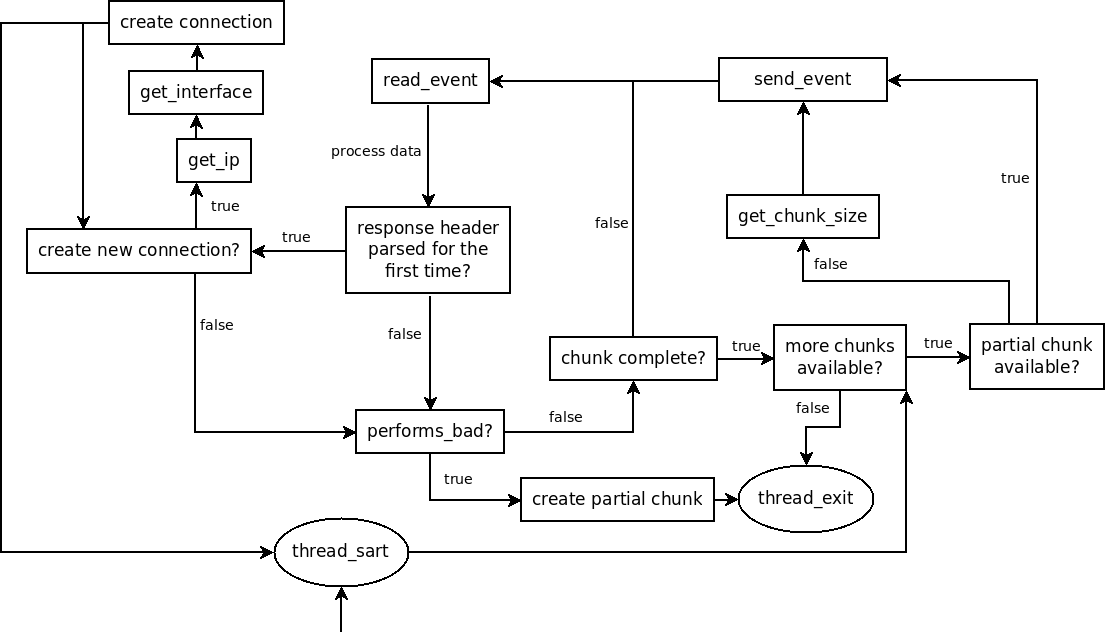
\includegraphics[width=0.48\linewidth]{Figures/scheduler_impl_1}
		\rule{35em}{0.5pt}
	\caption[Collector Thread]{Collector Thread Life Cycle \todo{do in latexdraw}.}
	\label{fig:scheduler_impl_1}
\end{figure}

The scheduler consists of two independent modules. 
First there is the path manager that decides which connection endpoints are chosen to establish a new path. 
Second there is the chunk size scheduler. 
It is making a decision for a request range $s$ for a connection $c$ over interface $i$ at time $j$.

\subsection{Path Manager Calls}
\label{sec:path-manager-calls}

\subsection{Scheduler Calls}
\label{sec:scheduler-calls}

In figure \ref{fig:scheduler_impl_1} the life cycle of a collector thread is depicted. 
A collector thread is responsible for sending requests and receiving the server responses.
During its runtime the thread is doing different calls to the scheduler and path manager interface in order to get instructions on how to behave next. 
By changing the underlying implementations later, we can implement different algorithms without touching the overlaying prototype implementation. 
The thread starts in the chunk management section. 
Here we determine whether or not more chunks need to be requested and what the chunk size is. 

When sending and receiving data the scheduler is notified in order to do proper link measurements. 
Upon receiving data or reaching a certain wait timeout, the thread asks the scheduler whether or not it should shut down due to performance issues. 
This is particularly important in case a path behaves very bad and we need to reschedule the chunk on another link. 
In that case, the already received data of that chunk will be stored and only the missing bytes will be re-requested. 
(TODO: put subsection into fluent text describing the figure)


%\subsection{Hook Set}
%\textbf{Metrics Determination}\newline
%void send\_event(void)\newline
%This hook is called each time prior to a thread making a chunk request. It is used to keep a timestamp to later estimate a rtt sample.\newline\newline

%void read\_event(size\_t bytes)\newline
%This hook is called each time a thread performed a socket read operation. It is used to keep track of the amount of bytes read and timestamps. Further in this function rtt (in case of first response read operation) and throughput $B$ are estimated.\newline\newline

%\textbf{Path Management}\newline
%unsigned long get\_ip()\newline
%This hook is called each time a thread wants to open a new socket. It returns the next suitable server $IP$ for the next path to open, meaning it determines the server endpoint for the next path.\newline\newline

%mpsock\_interface *get\_interface()\newline
%This hook is called each time a thread wants to open a new socket. It returns the interface the client should use for the next path, meaning it determines the client endpoint for the new connection.\newline\newline

%\textbf{Chunk Size}
%size\_t chunk\_size()\newline
%This hook is called each time a thread is preparing a new chunk request. Here is where the main work of the scheduling algorithm is done, since this is where we determine how to chunk our data.\newline\newline

%\textbf{Security Mechanisms}
%int performs\_bad()\newline
%This hook is called each time a thread performed a socket read operation. It determines whether this path is performing bad and whether it should shutdown or stay idle for a while. This is mainly used to avoid scenarios in which a bad performing connection stays busy while another good performing connection stays idle.\newline\newline

%int req\_over\_new\_connection()\newline
%This hook is called each time a thread is forced to stop using its current path. If true, the calling thread will open a new path to request the remaining chunks.
